\documentclass[tikz]{standalone}
\usetikzlibrary{patterns}
\begin{document}
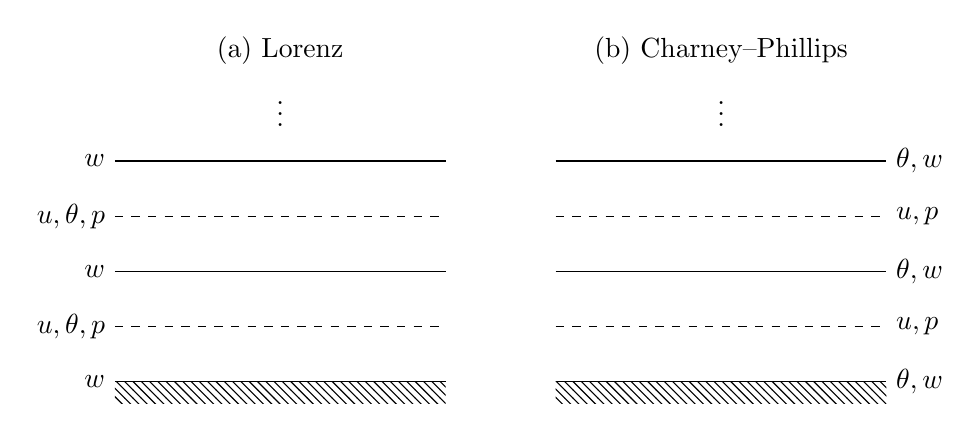
\begin{tikzpicture}[
  scale=0.7
]
\fill [pattern=north west lines] (0,0) rectangle (6,-0.4);
\fill [pattern=north west lines] (8,0) rectangle (14,-0.4);
\draw (0,0) -- (6,0) node [at start, anchor=east] {$w$};
\draw (8,0) -- (14,0) node [at end, anchor=west] {$\theta, w$};

\draw [dashed] (0,1) -- (6,1) node [at start, anchor=east] {$u, \theta, p$};
\draw [dashed] (8,1) -- (14,1) node [at end, anchor=west] {$u, p$};

\draw (0,2) -- (6,2) node [at start, anchor=east] {$w$};
\draw (8,2) -- (14,2) node [at end, anchor=west] {$\theta, w$};

\draw [dashed] (0,3) -- (6,3) node [at start, anchor=east] {$u, \theta, p$};
\draw [dashed] (8,3) -- (14,3) node [at end, anchor=west] {$u, p$};

\draw (0,4) -- (6,4) node [at start, anchor=east] {$w$};
\draw (8,4) -- (14,4) node [at end, anchor=west] {$\theta, w$};

\node at (3,5) {$\vdots$};
\node at (11,5) {$\vdots$};

\node at (3,6) {(a) Lorenz};
\node at (11,6) {(b) Charney--Phillips};
\end{tikzpicture}
\end{document}
